\section{Baseline-only state-response development}

This build tests main-effect transfer before expanding the architecture. Matched-control-relative effects, source-only inner selection and whole-biological-group outer folds define the task. Query treatment outcomes never fit control PCA, target means or response bases. The source control panels permit explicitly declared query-control gene selection; fitted state encodings remain source-only.

The corrected scPerturb 1.4 sci-Plex 3 release is publisher-MD5 verified \citep{srivatsan2020state,scperturb2024state}. Its full matrix has 799,317 rows, including unassigned cells and a separate 72-hour A549 block. Restricting to 24-hour human-cell-line conditions, 24 shared exact 1,000-nM intervention identities yield 144 single condition means across 24 line/plate strata and three biological line groups. All plates and replicates of a line remain on one side of each holdout. The 512 human-gene panel uses controls only; count-library normalization uses human genes. Wells receive equal weight, and each effect subtracts its own line/plate-matched vehicle. Plate count is not independent state replication.

\begin{table}[ht]\centering\small\begin{tabular}{lrrr}\toprule Source & Target mean & Selected simple & Learned state \\ \midrule

EmeraldBay & 0.064758 & 0.064680 & 0.073678 \\

sci-Plex 3 & 0.074913 & 0.074906 & 0.091868 \\

\bottomrule\end{tabular}\caption{Nested main-effect context development. Each source has its own scale/vocabulary and fixed evaluation population; MSE is not compared between sources. Neither simple-state nor learned-representation comparison passes the registered 5\% gate.}\end{table}

\begin{figure}[ht]\centering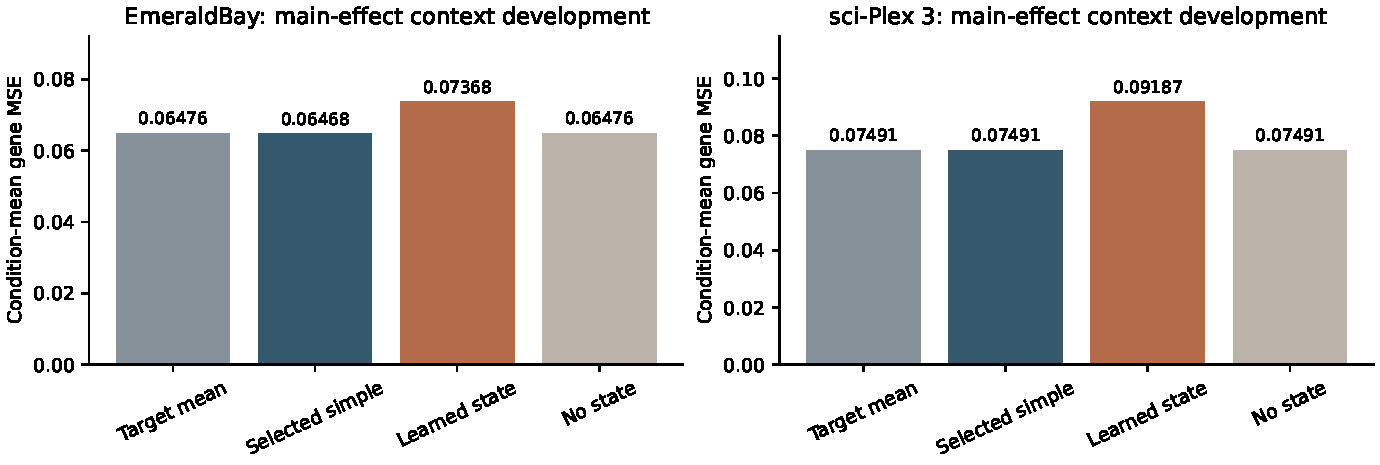
\includegraphics[width=\linewidth]{evidence/state_main.pdf}\caption{Source-average anchors remain strong. Removed-state and shuffled-input controls use the same supervision and output anchor; they are encoder ablations, not unseen-intervention methods.}\end{figure}

State-conditioned simple references improve on target averaging by 0.121\% on EmeraldBay and 0.010\% on sci-Plex 3. The learned candidates are respectively 13.91\% and 22.65\% worse than selected simple references. These negative development results close the scaling/routing gate for this build; three sci-Plex lines do not support a broad state-generalization conclusion.

Nominal sci-Plex duplicate-well profiles have mean replicate-difference MSE 0.063736, compared with a mean selected-simple improvement of 0.00000718. The replicate contrast includes plate and biological variation, shared controls and estimation error; it is a measurement-sensitivity comparison, without an identified biological accuracy ceiling or independent-culture precision claim.

\subsection{State-dependent residual and training-stage comparisons}

Only EmeraldBay source-development pair outcomes enter this new experiment; historical pair calibration and evaluator outcomes are not reopened. Inner kernel selection masks query singles and uses the same estimated-single route as outer evaluation. Symmetric sum/difference and product heads train measured-single residuals with the main model fixed. Joint variants retain source-single supervision and independent held-single diagnostics. Frozen and fine-tuned encoders use two residual seeds and equal pair epochs; removing neural single pretraining retains the source-average anchor and bases.

\begin{table}[ht]\centering\small\begin{tabular}{lrrrr}\toprule Model & Total & Main & Residual & Cross term \\ \midrule

Estimated additive & 0.18978 & 0.18380 & 0.19237 & -0.18639 \\

Selected kernel & 0.09461 & 0.18380 & 0.17046 & -0.25966 \\

Staged state & 0.11239 & 0.18380 & 0.16674 & -0.23815 \\

Frozen-encoder joint & 0.10163 & 0.17534 & 0.15817 & -0.23188 \\

Fine-tuned joint & 0.10148 & 0.17519 & 0.15755 & -0.23126 \\

No neural pretraining & 0.09516 & 0.16712 & 0.15721 & -0.22917 \\

\bottomrule\end{tabular}\caption{Pair/context development on one fixed population. Total error equals main plus residual error plus the cross term. Large negative cross terms prevent interpreting good total error as accurate interaction recovery.}\end{table}

\begin{figure}[ht]\centering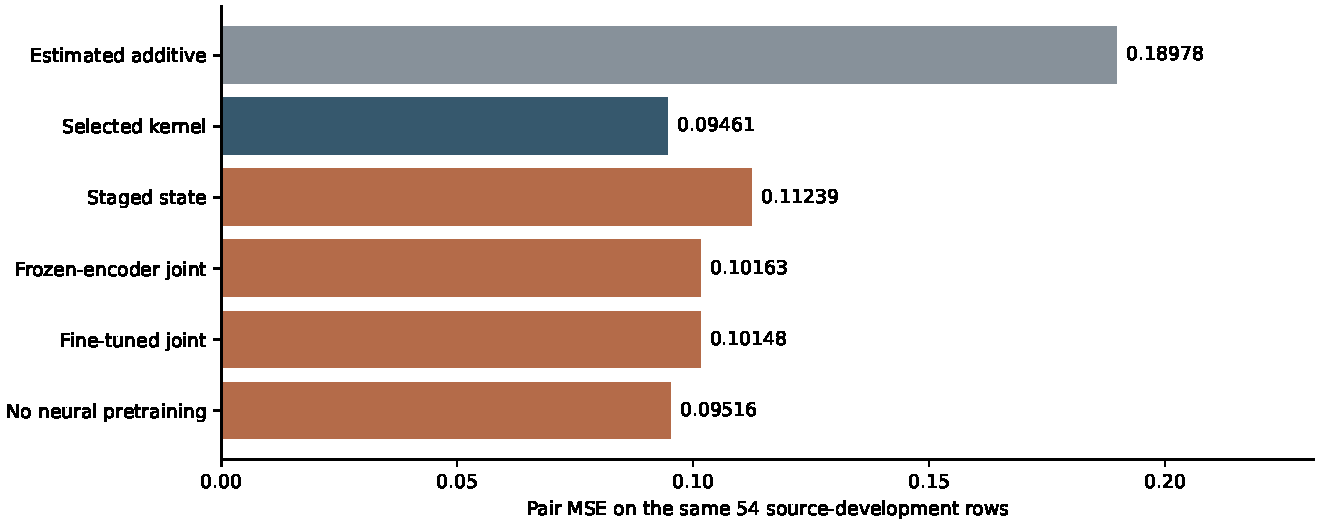
\includegraphics[width=0.98\linewidth]{evidence/state_pairs.pdf}\caption{State heads improve their pooled neural counterparts, but none beats the information-matched selected residual kernel. No winner is selected retrospectively from these outer scores.}\end{figure}

\subsection{Reliability, resources and remaining evidence}

A risk diagnostic fits separately from two-group calibration and two-group evaluation. At nominal 90\%, two calibration groups cannot produce a finite group-rank radius. Accept-none and accept-all comparisons remain visible; the registered accepted-risk/coverage criterion also fails. This is shared-study development, not fresh risk confirmation. D-SPIN remains a failed transfer of the earlier source radius. Inference returns unavailable intervals and diagnostic support rather than a confidence percentage.

Three subset orders retune simple references at each context budget with fixed query conditions. These dependent retrospective curves and hypothetical condition-assay costs do not establish prospective acquisition value. A new uncertainty-based acquisition extension is withheld after failed gates. Native CPA/GEARS results remain information-scoped historical comparisons; full-gene PertAdapt remains unscored. A separately identified 256-token synthetic adapter probe passes float32, float16 and bfloat16 forward/backward at batches one and two, without proving full-gene memory fit. A Linux/NCCL system with full gene alignment and an initial 48-GB float32 profiling budget is the documented next compute target, not an authorized purchase.

Two-seed portable NumPy exports preserve normalization, gene order, exact-condition records, supporting reference identities and all heads. The complete suite passes 115 tests. Python and CLI routes validate compatible previously unregistered baselines, pair swapping and one-time baseline reconstruction outside the checkout in an isolated installation. Engineering completion does not establish independent confirmation or reliable inference. A replicated, randomized shared-intervention screen with separate sealed confirmation and risk-calibration blocks remains required.
